\section{Sensor Node Hardware}

\begin{figure}
 \centering
 \begin{minipage}{0.8\linewidth}
 \centering
 \includegraphics[width=1\linewidth]{images/IMG_7354-01.eps}
  \caption[Wireless Sensor Node Prototype]{Wireless Sensor Node Prototype.}
  \label{fig:prototype}
 \end{minipage}
\end{figure}

The sensor node is comprised of two main parts, seen in Figure~\ref{fig:arch}. The primary intent of the sensor node is obviously to sense something and therefore the sensor or sensors make up one of those parts. Our sensor node uses magnetoresistive sensors to sense the magnetic field and it is sensitive enough to detect field in the range of at least tens of nanotesla. The prototype can be seen in Figure~\ref{fig:prototype}. In order to understand why we have chosen anisotropic magnetoresistors we have to look at the arguments for and against other systems.

\begin{figure}[thbf]
 \centering
 \begin{minipage}{0.8\linewidth}
 \centering
  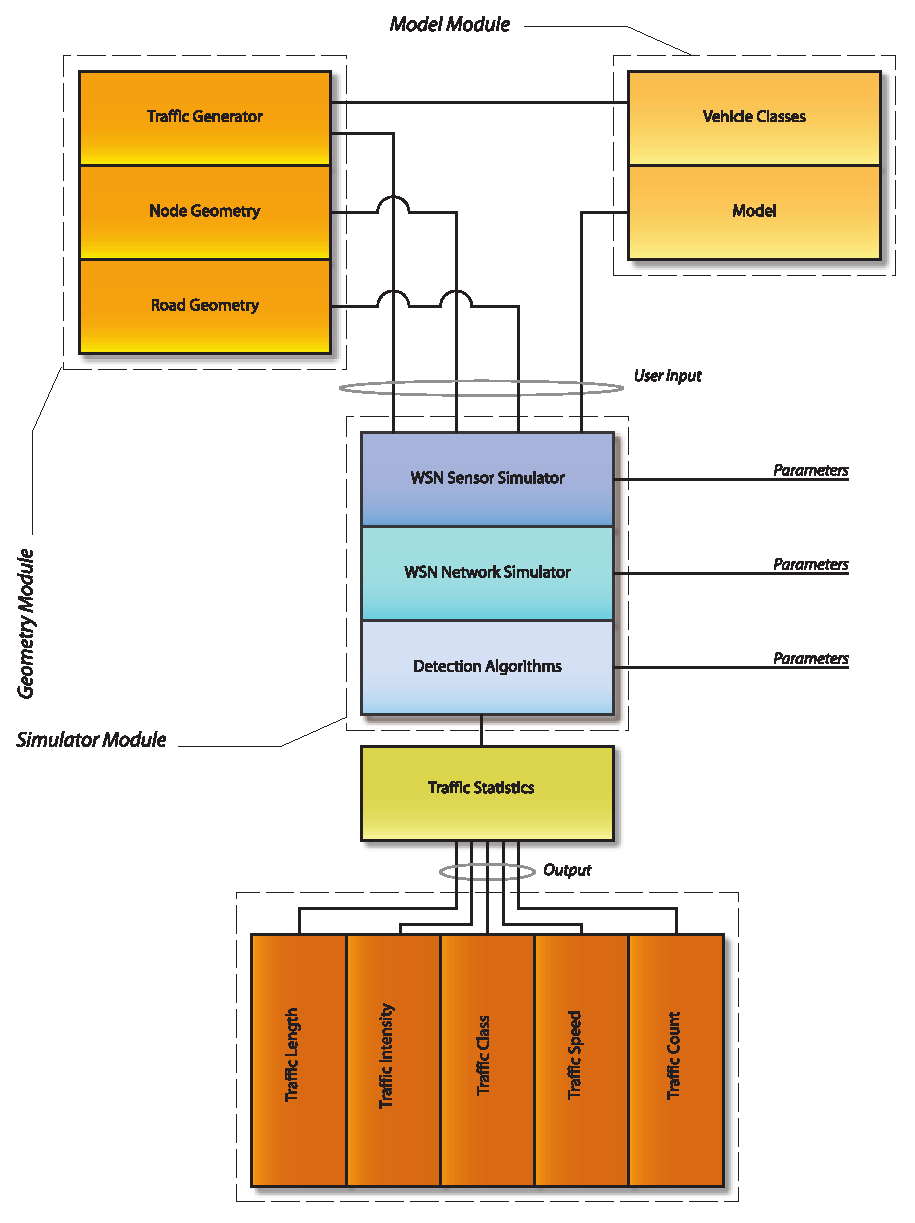
\includegraphics[width=1\linewidth]{images/architecture}
  \caption[Wireless Sensor Node Architecture]{Wireless Sensor Node Architecture.}
  \label{fig:arch}
 \end{minipage}
\end{figure}

% \section{What came in the beginning?}

\subsection{Comparison of existing technologies}
The different surveillance technologies can be classified as intrusive\index{surveillance technologies!intrusive}, non-intrusive\index{surveillance technologies!non-intrusive} or off-roadway\index{surveillance technologies!off-roadway}~\cite{path2007}. Intrusive sensor systems are installed in or on the pavement, non-intrusive are installed over or at the side of the road. Off-roadway systems are special since they need no equipment installed on-site.

\subsubsection{Inductive loop}\index{inductive loop}
The energy is used for measuring change in oscillator frequency~\cite{path2007} over the sensor loop and for analog to digital (A/D) conversion~\cite{cheung2005-2}. The inductive loop\index{inductive loop} is therefore an active sensor. Inductive loops are today the most common vehicle detector in use and is today a mature technology. It has a high detection accuracy. The disadvantages include high-cost installation and traffic disruption during installation. The loop wire is affected by stresses in the road surface and temperature making the failure rate high~\cite{path2007}.

\subsubsection{Pneumatic Tube}\index{pneumatic tube}
A pneumatic tube system is a very basic system that uses pressurised tubes to measure traffic parameters. When a vehicle passes the tube a pulse of air pressure is transferred along the tube. The output is therefore only detection, however with more than one tube, you can find the speed and even classify vehicles. The simplicity of this system is apparent. One of the major drawbacks, especially in Sweden, is that measurements can not be done in the winter time due to the possibility that the tubes will be plowed away by snow plows.

Installation and maintenance costs are kept low due to its simplicity. Drawbacks include inaccuracy in axle counting when buses and trucks are common~\cite{path2007}. The sensitivity is temperature dependant, and the equipment wear and tear is significant. 

\subsubsection{Piezoelectric sensor}\index{piezoelectric sensor}
A piezoelectric sensor uses a material that will generate an electrical potential when mechanical stress is applied. The output is proportional to the force applied and is only present when the force is changing. Classification is done here by axle count, spacing and vehicle weight. These types of sensors also have high-cost installation and maintenance. 

\subsubsection{Weigh-In-Motion system}\index{Weigh-In-Motion system}
A Weigh-In Motion (WIM) system will estimate the gross weight of a passing vehicle using different types of technology embedded in the road or on the road. These sensors can be of the piezoelectric type described previously. They can also depend on a capacitance mat, on hydraulic fluid in a pressure transducer (load cell sensor\index{load cell sensor}) or fiberoptics. A fiberoptic system is popular since it is installed by sticking thin tubes onto the pavement as opposed to burying the sensors~\cite{path2007}.

\subsubsection{Infrared-based system}\index{infrared-based system}
An infrared-based system can be either passive or active. A passive system relies on the emitted radiation from vehicles and ground surfaces while an active system uses the time difference between transmit and receive of the reflected pulse. The performance of the system is greatly affected by the environment, for example rain and snow, sunlight and temperature.

\subsubsection{Ultrasonic system}\index{ultrasonic system}
Ultrasonic sound waves are used for ranging in these systems and the principle is similar to that of a radar. There are models using Doppler shift\index{Doppler shift} to measure speed. Disadvantages include temperature and wind dependence~\cite{path2007}.

\subsubsection{Passive acoustic system}\index{passive acoustic system}
By using an array of microphones, the acoustic energy produced by a vehicle is measured. Performance is affected by temperature and accuracy drops with slow moving vehicles~\cite{path2007}.

\subsubsection{Video Image Processing}\index{Video Image Processing}

A video traffic detection system relies on image processing of optical data and therefore it is affected by weather conditions and lighting conditions. The system can also be affected by traffic intensity, and camera placements since vehicles in the background will make it harder for the image processing algorithms. 

\subsubsection{Microwave Radar}\index{microwave radar}

A radar system works in the same way as a video system but since it is not using optical wavelengths it is not affected by weather and lighting conditions to the same degree. It is however affected by traffic intensity and radar sensor placement.
There are a number of different types of radar systems, each with its advantages and disadvantages. A continuous wave\index{microwave radar!continuous wave} (CW) radar estimate the vehicle speed with the use of a single radar sensor. With the use of frequency-modulated continuous wave\index{microwave radar!frequency-modulated continuous wave} (FMCW) radar, a pair of of radar zones must be used.

\subsubsection{Off-roadway technologies}
These systems do not need any roadside hardware. Technologies include Global Positioning System\index{GPS} (GPS) positioning of mobile phones and Automatic Vehicle Identification\index{Automatic Vehicle Identification} (AVI). Positioning by mobile phones is interesting because it is rare that any vehicle do not have a mobile phone so no equipment need to be installed. Remote sensing by satellite or aircraft, optical or radar, can be used but has limited coverage due to the low availability of aircraft and satellites.

\subsection{Summary of different technologies}
In Tables~\ref{tbl:techs} and~\ref{tbl:enviromentaleffects} a comparison between the different technologies are presented. In Table~\ref{tbl:techs} we can see the capabilities of the different systems and in Table~\ref{tbl:enviromentaleffects} we can find what affects their performance. There is of course a big difference in installation cost and maintenance costs for these systems and the data they produce differ in accuracy. Inductive loops, which are the most used today, have a very good accuracy but are expensive. A WSN also has a good accuracy but is much cheaper, and can outperform the inductive loop. There are also differences within the same system. For example a side-fire or overhead-fire VIP system has much different performance.

\begin{table}[!f]
\centering
\caption[Capabilities of different technologies]{Capabilities of different technologies~\cite{path2007}.}
\begin{tabular}{lccccc}\toprule
	\textbf{Technology} 	& \textbf{Presence} & \textbf{Count} & \textbf{Direction} & \textbf{Speed} & \textbf{Classification}\\\midrule
	Pneumatic tube		&		& $\bullet$	& $\bullet$	& $\bullet$	& Wheel axes\\
	Piezoelectric sensor	&		& $\bullet$	& $\bullet$	& $\bullet$	& Wheel axes\\
	WIM system		& $\bullet$	& $\bullet$	& $\bullet$	& $\bullet$	& Wheel axes\\
	CW radar		& 		& $\bullet$	& $\bullet$	& $\bullet$	& \\
	FMCW radar		& $\bullet$	& $\bullet$	& $\bullet$	& $\bullet$	& Shape\\
	Active infrared		& $\bullet$	& $\bullet$	& $\bullet$	& $\bullet$	& Shape\\
	Passive infrared	& $\bullet$	& $\bullet$	& $\bullet$	& $\bullet$	& Shape\\
	Video Image Processing 	& $\bullet$	& $\bullet$	& $\bullet$	& $\bullet$	& Shape\\
	Ultrasonic		& $\bullet$	& $\bullet$	& $\bullet$	& $\bullet$	& Shape\\
	Passive Acoustic	& $\bullet$	& $\bullet$	& $\bullet$	& $\bullet$	& Sound\\
	Inductive loop		& $\bullet$	& $\bullet$	& $\bullet$	& $\bullet$	& Magnetic signature\\ 
	AMR Sensors		& $\bullet$	& $\bullet$	& $\bullet$	& $\bullet$	& Magnetic signature\\ \bottomrule
\end{tabular} 
\label{tbl:techs}
\end{table} 

\begin{table}[!f]
\centering
\caption[Sensitivity of technologies to environmental effects]{Sensitivity of technologies to environmental effects~\cite{path2007}.}
\begin{tabular}{lcccc}\toprule
 \textbf{Technology} 	& \textbf{Wind} & \textbf{Temperature} & \textbf{Lighting} & \textbf{Traffic flow}\\\midrule
 Inductive loop		& 		& $\bullet$	& 		&	\\
 Pneumatic tube		& 		& $\bullet$	&		& $\bullet$	\\
 Piezoelectric sensor	& 		& $\bullet$	&		&	\\
 WIM system		& 		& 		& 		& 	\\
 CW radar		& 		& 		& 		& $\bullet$ 	\\
 FMCW radar		& 		& 		& 		& 	\\
 Active infrared	& 		&		&		& 	\\
 Passive infrared	& 		& 		& 		& 	\\
 Video Image Processing & 		& $\bullet$	& $\bullet$	& 	\\
 Ultrasonic		& $\bullet$	&		&		& 	\\
 Passive Acoustic	& $\bullet$	& $\bullet$	& 		& $\bullet$	\\
 AMR Sensors		& 		& $\bullet$	& 		& 	\\ \bottomrule
\end{tabular} 
\label{tbl:enviromentaleffects}
\end{table} 


\subsection{AMR Magnetic sensors}

Some materials change their electrical resistance when exposed to a magnetic field~\cite{imego2006}. This magnetoresistive effect\index{magnetoresistive effect} is used in anisotropic magnetoresistance sensors\index{anisotropic magnetoresistance sensor} (AMR)\index{AMR Sensor|see{anisotropic magnetoresistance sensor}} sensors. The resistive elements are most often made of nickel-iron~\cite{caruso1998} (Permalloy\index{Permalloy}) thin films.

The benefits of using this type of sensor come from its ability to sense static magnetic fields as well as the direction of those fields. The detection range is also suitable for our purposes. They are very sensitive to magnetic fields -- according to ~\cite{imego2006} they have a noise specification of in the order of  nT/$\sqrt{\text{Hz}}$ and one of the sensors we are using has a resolution of $2.7$~nT. As a comparison computer floppy disks store data with field strengths of approximately $1\cdot{}10^6$~nT~\cite{hmc2300}. Another important fact is that the sensors can be bulk manufactured on silicon wafers, and thus are cheaper.

In an AMR sensor these magnetorestive materials are used in a ``Wheatstone~bridge''~\cite{an218}\index{Wheatstone bridge}. A typical AMR sensor bridge can be seen in Figure~\ref{fig-barberpole} and the electrical diagram of a Wheatstone bridge can be seen in Figure~\ref{fig-wheatstone}. Each bridge has four resistive elements which are ordered so that opposite elements are equal. If a magnetic field is applied, two of the resistive elements will decrease slightly in resistance. The other two will increase slightly.

\begin{figure}
\centering
\begin{minipage}{1\linewidth}
 \centering
 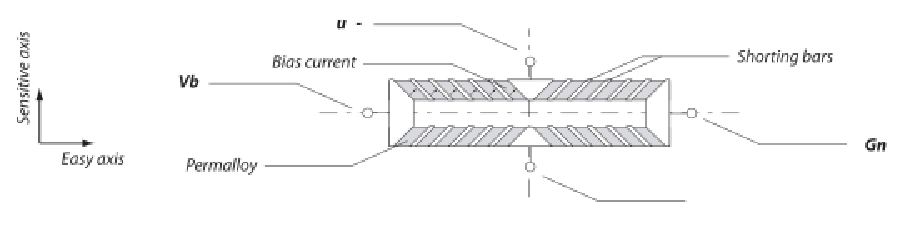
\includegraphics[width=1\linewidth]{images/barberpole}
 % wheatstone.eps: 1179666x1179666 pixel, 300dpi, 9987.84x9987.84 cm, bb=
 \caption[AMR Barber Pole Bias]{AMR Barber Pole Bias.}
 \label{fig-barberpole}
\end{minipage}
\end{figure}

\begin{figure}
\centering
\begin{minipage}{0.3\linewidth}
 \centering
 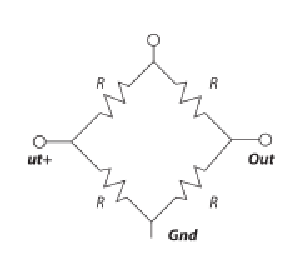
\includegraphics[width=1\linewidth]{images/wheatstone}
 % wheatstone.eps: 1179666x1179666 pixel, 300dpi, 9987.84x9987.84 cm, bb=
 \caption[Wheatstone bridge]{Wheatstone bridge\index{Wheatstone bridge}. Voltage difference between \emph{OUT+} and \emph{OUT-} is measured.}
 \label{fig-wheatstone}
\end{minipage}
\end{figure}

The voltage between the out terminals $\text{Out}_{+}$ and $\text{Out}_{-}$ on the sensor is measured. That voltage is dependant on the sensor sensitivity, the bridge supply voltage and the applied field~\cite{an218}. 
 
\begin{equation}
 \text{Out}_{+}\,-\,\text{Out}_{-} = SV_bB_s,
\end{equation}

where $S$ is the sensor sensitivity  [mv/V/T], $V_b$ the bridge supply voltage and $B_s$ the applied magnetic field [T].
In order to detect a magnetic field of any orientation we will need three of these sensors -- one for each axis. 

The properties of the AMR sensor are only well-behaving when the magnetic domains of the film is aligned with each other. The ``easy~axis''\index{easy axis} of the magnetisation vector $\vec{M}$ is set during fabrication, see Figure \ref{fig-amrnoapplied}. The $\vec{M}$ vector is then parallel to the length of the resistor. The low-resistance shorting bars (seen in Figure~\ref{fig-barberpole}) is there to make the current flow at a 45 degree angle to the film which gives us an angle $\theta$ between the current vector and the magnetisation vector. The resistance is dependent on the angle $\theta$ and reaches its maximum when the current vector is parallel to the magnetisation vector~\cite{caruso1998}. The technique for producing this ``shortest path'' through the resistor is called barber pole biasing.

\begin{subfigures}
\begin{figure}[!ht]
  \centering
  \begin{minipage}{0.3\linewidth}
  \psfrag{Magnetisation}{\tiny{}Magnetisation}
  \psfrag{t}{$\theta$}
  \centering
   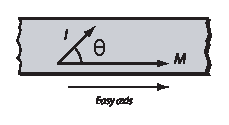
\includegraphics[height=1.5cm]{images/amrnoapplied}
  \caption[Magnetoresistive effect. Permalloy resistor, no applied field]{Magneto\-resistive effect. Perm\-alloy (NiFe) res\-i\-st\-or~\cite{caruso1998}, no app\-lied field.}
  \label{fig-amrnoapplied}
  \end{minipage}\hspace{0.5cm}
   \begin{minipage}{0.3\linewidth}
  \psfrag{Magnetisation}{\tiny{}Magnetisation}
  \psfrag{t}{$\theta$}
  \centering
   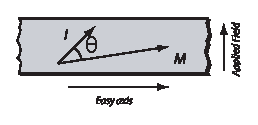
\includegraphics[height=1.5cm]{images/amrapplied}
  \caption[Magnetoresistive effect. Permalloy resistor, applied field]{Magnetoresistive effect. Permalloy resistor, applied field.}
  \label{fig-amrapplied}
  \end{minipage}
 \end{figure}
\end{subfigures}

If we now apply a magnetic field normal to the easy axis the magnetisation vector will rotate and we will see a change in the voltage output of the Wheatstone bridge. The magnetoresistive effect is directly related to the angle $\theta$~\cite{hmc1001}. See Figure~\ref{fig-amrapplied}.

A magnetic field will break down the alignment of the magnetisation vector which is essential to receive accurate measurements. The resistor is made up of many magnetic domains whose magnetisation vector can point in any direction, see Figure~\ref{fig-amr1}. For small disturbances, these magnetic domain magnetisation vectors will rotate back to their previous direction when the field is no longer applied. For large fields however they will not. To realign the total magnetisation vector with the easy axis we can apply a strong magnetic field in the right direction. The Honeywell sensors are for this reason equipped with a Set/Reset (S/R) strap that can be pulsed with high current to reset the sensor and align the magnetisation vector with the easy axis again. The effect of the S/R pulses can be seen in Figure~\ref{fig-amr2} and~\ref{fig-amr3}.
 
\begin{subfigures}
\begin{figure}[!ht]
  \centering
  \begin{minipage}{0.3\linewidth}
\psfrag{Easy axis}{\tiny{}Easy axis}
  \centering
   
\includegraphics[height=1.5cm]{images/amr1}
  \caption[Magnetic moment domain orientations]{Random magnetic do\-main orient\-a\-tions~\cite{hmc1001, an213} before set/reset pulse. Note the sens\-itive axis.}
  \label{fig-amr1}
  \end{minipage}\hspace{0.5cm}
  \begin{minipage}{0.3\linewidth}
  \psfrag{Magnetisation}{\tiny{}Magnetisation}
  \centering
   
\includegraphics[height=1.5cm]{images/amr2}
  \caption[Magnetic moment domain orientations after a set pulse]{Magnetic moment domain orientations after a set pulse~\cite{hmc1001, an213}. Moments aligned to the right.}
  \label{fig-amr2}
  \end{minipage}\hspace{0.5cm}
   \begin{minipage}{0.3\linewidth}
  \psfrag{Magnetisation}{\tiny{}Magnetisation}
  \centering
   
\includegraphics[height=1.5cm]{images/amr3}
  \caption[Magnetic moment domain orientations after a reset pulse]{Magnetic moment domain orientations after a reset pulse~\cite{hmc1001, an213}. Moments aligned to the left.}
  \label{fig-amr3}
  \end{minipage}
 \end{figure}
\end{subfigures}
 
\begin{figure}
\centering
\begin{minipage}{0.4\linewidth}
 \centering
 \psfrag{t}{$\tau$}
 \psfrag{tpw}{$\tau_{\text{\tiny PW}}$}
 \includegraphics[width=1\linewidth]{images/set-reset}
 \caption[Set/Reset pulses for magnetic sensor]{Set/Reset pulses of HMC100x, HMC1043.}
 \label{fig-setreset}
\end{minipage}
\end{figure}

We need to create the current through the S/R strap and this is done using an H-bridge. The current pulse shape can be seen in Figure~\ref{fig-setreset}. The S/R current has a high power requirement. We need to minimise the current, and maximise the time between the S/R pulses in order to conserve battery power. A number of schemes for doing this has been tested, among those are

\begin{itemize}
 \item Use only set or reset pulse at any time, interchange them,
 \item Use less current for each pulse,
 \item Maximise the time between pulses,
 \item Only S/R when a high field has been present.
\end{itemize}

It is most likely that a combination of the above will produce the best result. An important parameter in this is the usage of the sensor. If we need to detect small fields, then we need to do this more often. 

\section{Sensor Hardware}\label{cha:hardware}

The sensor nodes should be inexpensive, battery powered (maybe with an option for an external power source), rugged, easy to maintain, and easy to install. A prototype sensor node has been built by a previous project~\cite{arrigault2007} at Qamcom~Technology~AB. 

The sensor should be easy to operate, be capable of near-real-time calculations and withstand road conditions in the most demanding of climates. Here in Sweden the climate offer snow and ice in the winter and high temperatures in the summer. It should be able to operate for a long time in these climates putting enormous strain on the power supply. The power supply can be internally or parasitically powered.